\chapter{Pengenalan Cloud Computing dan Infrastruktur Pengembangan Aplikasi Berbasis Node.js}

\section{Apa itu Cloud Computing?}

Cloud Computing, \index{Cloud Computing} atau sering diterjemahkan sebagai ``Komputasi Awan'' dalam bahasa Indonesia mempunyai berbagai definisi:\index{Cloud Computing!Definisi}
\begin{itemize}
  \item \textbf{Wikipedia}: penggunaan sumber daya komputasi (peranti keras dan peranti lunak) yang berfungsi untuk memberikan layanan melalui suatu jaringan (pada umumnya Internet)\footnote{\url{http://en.wikipedia.org/wiki/Cloud_computing}}.
  \item \textbf{NIST\footnote{The National Institute of Standards and Technology}}: model yang memungkinkan akses jaringan ubiquitous (dari mana saja), nyaman, on-demand (saat ada permintaan) ke sekumpulan sumber daya komputasi yang dikonfigurasi untuk berbagi (jaringan, server, penyimpanan, dan berbagai layanan lain) yang dapat dengan cepat ditetapkan dan dirilis dengan usaha yang minimal dari manajemen ataupun interaksi dengan penyedia layanan\footnote{\url{http://csrc.nist.gov/publications/PubsSPs.html\#800-145}}.
\end{itemize}

Jika diwujudkan secara visual, Cloud Computing bisa dilihat pada Gambar~\ref{fig:ccsam}\footnote{Gambar dibuat oleh Sam Johnston, diambil dari \url{http://en.wikipedia.org/w/index.php?title=File:Cloud_computing.svg&page=1}}

  \begin{figure}[t]
    \begin{center}
      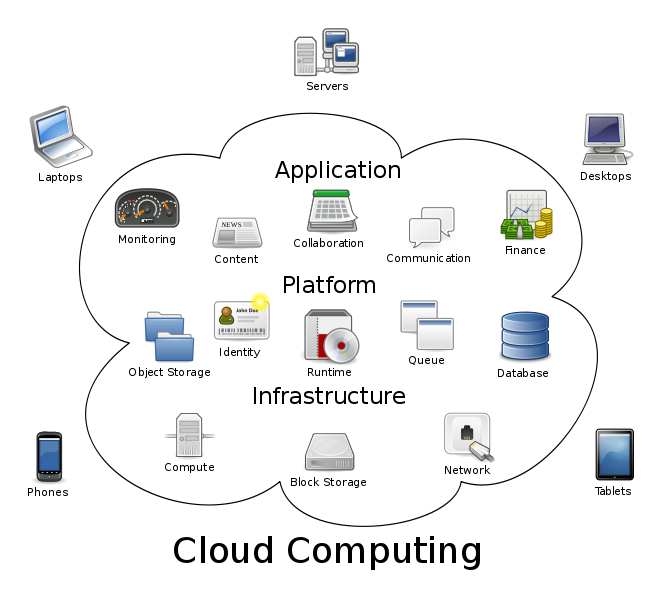
\includegraphics[scale=0.5]{images/662px-Cloud_computing.png}
    \end{center}
    \caption{Model Cloud Computing}
    \label{fig:ccsam}
  \end{figure}

\section{Karakteristik Cloud Computing}

Menurut NIST, ada beberapa karakteristik dari Cloud Computing:\index{Cloud Computing!Karakteristik}
\begin{itemize}
  \item \textbf{On-demand self-service}: layanan bisa diperoleh pada saat diminta, tanpa intervensi atau interaksi manusia di sisi penyedia jasa. 
  \item \textbf{Broad network access}: tersedia melalui jaringan dengan berbagai peranti yang umum (komputer, tablet, HP, dan lain-lain)
  \item \textbf{Resource pooling}: sumber daya komputasi dari penyedia jasa terkumpul untuk melayani.
  \item \textbf{Rapid elasticity}: skalabilitas.
  \item \textbf{Measured service}: penggunaan sumber daya bisa diukur, di-monitor, dikendalikan, dan dilaporkan.
\end{itemize}

Karakteristik lain yang tidak kalah penting adalah \textit{multitenancy}. \textit{Multitenancy} merupakan suatu prinsip dalam arsitektur software. Pada arsitektur tersebut, satu instan dari software berjalan pada server, melayani banyak organisasi klien. Aplikasi dirancang untuk mempartisi data dan konfigurasinya secara virtual dan setiap organisasi klien tersebut bekerja dengan instan aplikasi virtual tersebut\footnote{\url{http://en.wikipedia.org/wiki/Multitenancy}}. \index{Multitenancy}

\section{\textit{Public} dan \textit{Private} Cloud Computing}

\index{Cloud Computing!Private}Cloud Computing bisa dibangun untuk keperluan pribadi suatu organisasi dan (secara legal) hanya bisa diakses oleh organisasi yang bersangkutan. Tipe tersebut dikenal dengan \textit{Private Cloud Computing}. \index{Cloud Computing!Public}Sementara itu, jika sumber daya Cloud Computing bisa diakses oleh publik (dengan hak akses yang sesuai), maka model tersebut dikenal sebagai \textit{Public Cloud Computing}. Pembahasan di buku ini adalah pembahasan tentang \textit{Public Cloud Computing} dan semua referensi tentang Cloud Computing di buku ini akan menunjuk pada \textit{Public Cloud Computing} kecuali dinyatakan lain.

\section{Model Layanan Cloud Computing}

\index{Cloud Computing!Model layanan}Model layanan pada Cloud Computing akan berkembang sesuai kebutuhan konsumen serta inovasi dari berbagai penyedia layanan. Saat ini, pada umumnya, ada tiga model layanan:
\begin{itemize}
  \item \textbf{SaaS} (\textit{Software as a Service}): layanan berupa aplikasi yang ditempatkan pada infrastruktur penyedia layanan, siap digunakan oleh konsumen.
  \item \textbf{PaaS} (\textit{Platform as a Service}): menyediakan layanan ke konsumen berupa platform untuk men-deploy aplikasi.
  \item \textbf{IaaS} (\textit{Infrastructure as a Service}): menyediakan layanan ke konsumen berupa berbagai sumber daya komputasi (pemrosesam, penyimpanan, jaringan, dan sumber daya fundamental lainnya).
\end{itemize}

Meski sampai saat ini, umumnya terdapat tiga model tersebut, beberapa model kelihatannya sudah mulai muncul, misalnya STaaS (\textit{Storage as a Service}), SECaaS (\textit{Security as a Service}), DaaS (\textit{Data as a Service}), TEaaS (\textit{Test Environment as a Service}), \textit{Desktop Virtualization}, APIaaS (\textit{API as a Service}).

\section{Pengembangan Aplikasi di Cloud Computing}

Pada umumnya, para pengembang aplikasi di Cloud Computing juga menggunakan pendekatan \textit{Agile Software Development} yang berbasis pada pengembangan secara iteratif untuk setiap \textit{milestone} (dalam iterasi analisis-desain-\textit{coding-testing-debugging}) mulai dari \textit{milestone} paling awal sampai software dirilis. Perbedaan paling mendasar hanyalah pada platform yang digunakan untuk \textit{deployment}, peranti pengembangan yang digunakan, serta utilitas untuk mengelola aplikasi yang di-\textit{deploy} pada instan di cloud.

Pengembangan aplikasi di Cloud Computing akan melibatkan peranti pengembang yang didukung oleh infrastruktur Cloud. Kita akan memerlukan PaaS untuk keperluan ini. Pada dasarnya pengembangan aplikasi akan meliputi siklus berikut:

\begin{itemize}
  \item \textit{Coding}
  \item Test di komputer lokal
  \item Upload ke server (dalam Cloud Computing, proses ini diistilahkan dengan ``\textit{push}''
  \item Edit - push
\end{itemize}

Jika pengembangan aplikasi dilakukan oleh tim, maka perlu adanya software untuk \textit{version control}, misalnya Git, mercurial, dan lain-lain. Setelah itu, aktivitas yang dilakukan biasanya terpusat pada \textit{push} (untuk mengupload instan dari aplikasi ke server) dan \textit{pull} (untuk mengambil instan aplikasi dari server).

\section{Node.js dan Cloud Computing}

\index{Node.js}Node.js merupakan salah satu peranti pengembang yang bisa digunakan untuk membuat aplikasi berbasis Cloud. Node.js dikembangkan dari \textit{engine} JavaScript yang dibuat oleh Google untuk browser \textit{Chrome / Chromium} (V8) ditambah dengan libUV serta beberapa pustaka internal lainnya. Dengan menggunakan Node.js, semua pengembangan akan dilakukan menggunakan JavaScript, baik pada sisi klien maupun server. Node.js dibuat pertama kali oleh Ryan Dahl (twitter.com/ryah) dan sampai saat ini dikembangkan oleh komunitas sebagai software bebas dengan pendanaan utama dari Joyent, perusahaan tempat Ryan Dahl bekerja.

\section{Layanan Hosting Aplikasi: CloudFoundry}

\index{CloudFoundry}Saat ini, mulai banyak penyedia layanan Cloud yang mendukung Node.js, diantaranya adalah CloudFoundry (\url{http://www.cloudfoundry.com}, selanjutnya akan kita sebut dengan CF). Buku ini akan menggunakan fasilitas dari CF. Daftar lengkap dari penyedia infrastruktur Node.js bisa dilihat pada \url{https://github.com/joyent/node/wiki/Node-Hosting}.\index{Node.js!Hosting}

\subsection{Pendaftaran}

Untuk menggunakan fasilitas dari CF, kita akan mendaftar lebih dahulu di URL \url{https://my.cloudfoundry.com/signup} sepert yang terlihat pada Gambar~\ref{fig:cfsignup}.

\begin{figure}[t]
    \begin{center}
      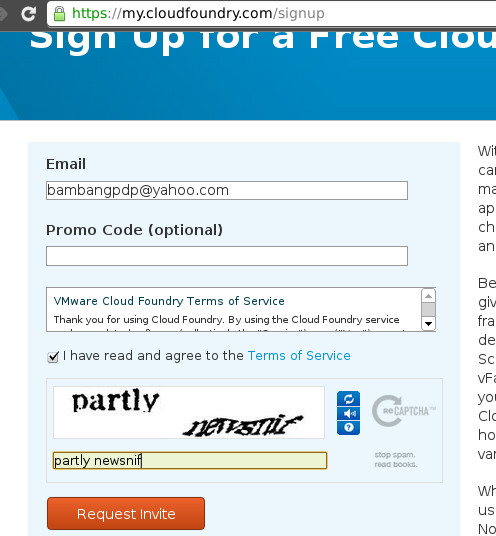
\includegraphics[scale=0.5]{images/cf-signup.jpg}
    \end{center}
    \caption{Pendaftaran di CF}
    \label{fig:cfsignup}
  \end{figure}

Setelah itu, CF akan mengirimkan pemberitahuan bahwa proses pendaftaran selesai seperti di Gambar~\ref{fig:cfsignuphasil}. \textit{Credentials} atau informasi tentang akun kita di CF akan dikirimkan ke e-mail kita seperti pada Gambar~\ref{fig:cfsignupapproved}.
 
  \begin{figure}
    \begin{center}
      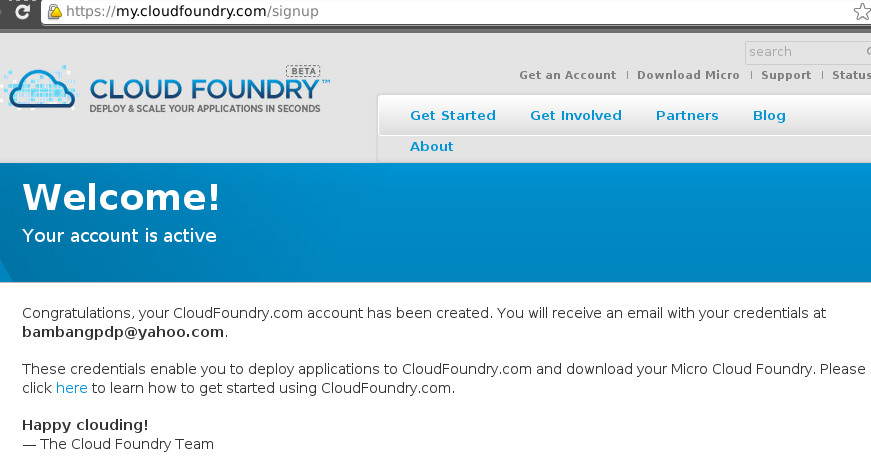
\includegraphics[scale=0.5]{images/cf-signup-hasil.jpg}
    \end{center}
    \caption{Hasil proses pendaftaran di CF}
    \label{fig:cfsignuphasil}
  \end{figure}

  \begin{figure}[t]
    \begin{center}
      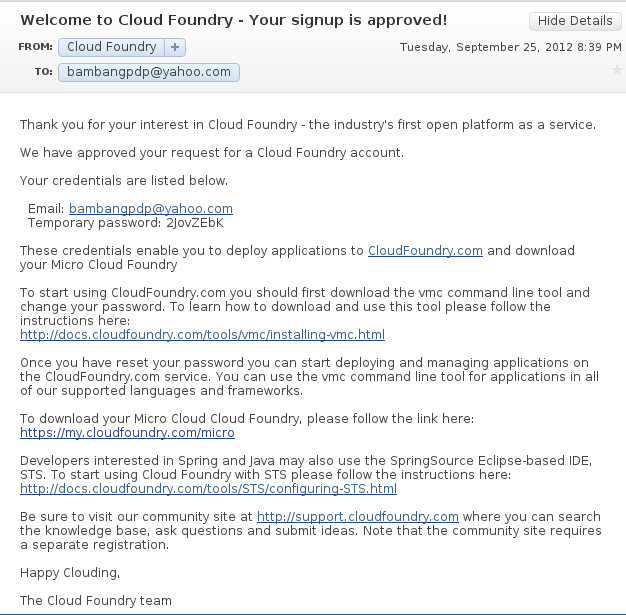
\includegraphics[scale=0.5]{images/cf-signup-approved.jpg}
    \end{center}
    \caption{E-mail persetujuan dan pemberitahuan \textit{credentials}}
    \label{fig:cfsignupapproved}
  \end{figure}

\subsection{Instalasi \textit{Command Line Utilities}}

\index{CloudFoundry!vmc}\textit{Command Line Utilities / CLU)} adalah software yang dijalankan melalui shell / \textit{command line / command prompt}. CLU untuk CF ini dibuat dengan menggunakan Ruby dan didistribusikan dalam bentuk \textit{gem} sehingga untuk instalasi ini diperlukan ruby dan rubygem. Berikut adalah perintah untuk instalasi vmc (CLU dari CF).

\lstset{language=bash,caption=Instalasi vmc}
\lstinputlisting{src/non-nodejs/bab-01/instalasi-vmc.txt}

Pesan peringatan berikut ini:

\lstset{language=bash,caption=Peringatan setting PATH untuk vmc}
\lstinputlisting{src/non-nodejs/bab-01/peringatan-setting-path-vmc.txt}

terjadi karena path untuk \textit{executable script} Ruby yang diinstall oleh vmc belum ditambahkan ke variabel lingkungan PATH. Edit file \$HOME/.bashrc dan tambahkan baris berikut\footnote{Catatan: "/home/bpdp/" adalah direktori \$HOME saya, silahkan sesuaikan dengan tempat anda}:
\lstset{language=bash,caption=Peringatan setting PATH untuk vmc}
\lstinputlisting{src/non-nodejs/bab-01/setting-path-vmc.txt}

Setelah itu, ketikkan di shell prompt Bash: \textit{source \~/.bashrc}\footnote{Ini hanya untuk keperluan saat ini saja, setelah ini tidak perlu lagi karena setiap login sudah akan dibaca oleh Bash}.

Hasil dari instalasi vmc adalah sebagai berikut:

\lstset{language=bash,caption=Hasil gem yang terinstall}
\lstinputlisting{src/non-nodejs/bab-01/gem-terinstall.txt}

Periksa dengan menjalankan opsi help dari vmc:

\lstset{language=bash,caption=Hasil opsi help dari vmc}
\lstinputlisting{src/non-nodejs/bab-01/vmc-help.txt}

\subsection{Konfigurasi di Server Cloud}

Pada dasarnya, yang diperlukan hanyalah mengubah target ke server cloud dari CF dan kemudian mengubah password.

\lstset{language=bash,caption=Mengubah target server - belum ada konfigurasi}
\lstinputlisting{src/non-nodejs/bab-01/vmc-target-no-conf.txt}

Error di atas terjadi karena file konfigurasi belum dibuat. File konfigurasi tersimpan di direktori \$HOME/.vmc. Mengubah target dilakukan dengan membuat file \textit{target} di direktori tersebut. Isi dari file target tersebut adalah server CloudFoundry, yaitu \textit{https://api.cloudfoundry.com}. Setelah itu, jika dieksekusi lagi, hasilnya adalah sebagai berikut:

\lstset{language=bash,caption=Mengubah target server - setelah konfigurasi}
\lstinputlisting{src/non-nodejs/bab-01/vmc-target-with-conf.txt}

Setelah itu, setiap kali kita akan melakukan berbagai proses yang melibatkan server ini, kita harus melakukan proses login terlebih dahulu:

\lstset{language=bash,caption=Login ke server}
\lstinputlisting{src/non-nodejs/bab-01/vmc-login-info.txt}

Untuk mengubah password:

\lstset{language=bash,caption=Mengubah password server}
\lstinputlisting{src/non-nodejs/bab-01/vmc-ubah-password.txt}

\subsection{Instalasi dan Konfigurasi Node.js di Komputer Lokal}

Node.js tersedia untuk Linux, Windows, Mac OS X, serta SunOS. Untuk versi Linux, kebanyakan distro sudah menyertakan paket Node.js, hanya saja ada banyak versi dari Node.js dan jika kita menggunakan manajemen paket dari distro Linux, kita hanya bisa menginstall 1 versi saja. Sebagai contoh, di Arch Linux, paket Node.js bisa diinstrall dengan perintah ``pacman -S nodejs'' tetapi hanya pada versi resmi di repo Arch Linux (versi 0.8.16 pada tanggal 7 Januari 2012). 

Langkah instalasi berikut ini adalah langkah untuk instalasi tanpa manajemen paket dari distro Linux.
\begin{itemize}
  \item Ambil paket \textit{binary executable} dari \url{http://nodejs/download} atau langsung ke \url{http://nodejs.org/dist/}. Versi yang digunakan disini adalah 0.8.16. Download file tersebut, kemudian simpan di direktori tertentu (terserah anda, dibuku ini diletakkan di \$HOME/master/nodejs).

\lstset{language=bash,caption=Hasil dari download Node.js}
\lstinputlisting{src/non-nodejs/bab-01/hasil-download-nodejs.txt}

  \item Ekstrak ke direktori yang diinginkan. Node.js akan diinstall di direktori \$HOME/software:

\lstset{language=bash,caption=Ekstraksi Node.js}
\lstinputlisting{src/non-nodejs/bab-01/ekstraksi-nodejs.txt}

  \item Konfigurasi variabel lingkungan. Sebaiknya disimpan pada suatu file (pada buku ini, konfigurasi akan disimpan di \textit{\$HOME/environment/nodejs}):

\lstset{language=bash,caption=Konfigurasi variabel lingkungan Node.js}
\lstinputlisting{src/non-nodejs/bab-01/konfigurasi-var-lingkungan-nodejs.txt}

  \item Setiap akan menggunakan Node.js, yang diperlukan adalah men-source file konfigurasi tersebut: \textbf{source \~/environment/nodejs}.
\end{itemize}

\section{Pengelolaan Aplikasi di Cloud}

Aplikasi yang dibuat nantinya akan di-deploy ke server CF. Pada umumnya, developer akan melakukan proses untuk upload (\textit{push}), menghapus (\textit{delete}), serta memperbaharui (\textit{update}) aplikasi di server. Jika belum memahami sintaksis JavaScript serta penggunaan npm, jangan kuatir. Tujuan dari bab ini hanya mengenalkan pengelolaan aplikasi di Cloud. Aspek lainnya akan dibahas di bab-bab berikutnya.

\subsection{\textit{Push, Delete, Update} Aplikasi}

Pada pembahasan ini, akan diberikan contoh menggunakan dua kategori, yaitu dengan menggunakan \textit{framework} (ExpressJS - \url{http://expressjs.com}) serta tanpa menggunakan \textit{framework}.

\subsection{Menggunakan Framework ExpressJS}

\lstset{language=bash,caption=Instalasi ExpressJS menggunakan npm}
\lstinputlisting{src/non-nodejs/bab-01/instalasi-expressjs.txt}

Jika berhasil, maka kita bisa menggunakan perintah \textit{express} untuk membuat rerangka aplikasi. Sintaksis penggunaan ExpressJS adalah sebagai berikut:

\lstset{language=bash,caption=Perintah express}
\lstinputlisting{src/non-nodejs/bab-01/express-help.txt}

Setelah itu, kita bisa membuat rerangka aplikasi ExpressJS dengan cara berikut:

\lstset{language=bash,caption=Menggunakan express untuk membuat rerangka aplikasi}
\lstinputlisting{src/non-nodejs/bab-01/express-buat-app.txt}

Pada rerangka aplikasi tersebut, terdapat file \textit{package.json} untuk mendefinisikan aplikasi serta dependensi-nya dan app.js yang merupakan file utama untuk dijalankan pada server.

\lstset{language=Javascript,caption=package.json untuk ExpressJS}
\lstinputlisting{src/bab-01/hello-vanilla/package.json}

\lstset{language=Javascript,caption=app.js untuk ExpressJS}a
\lstinputlisting{src/bab-01/hello-vanilla/app.js}

Edit file \textit{routes/index.js} sebagai berikut:

\lstset{language=Javascript,caption=Hasil edit routes/index.js}
\lstinputlisting{src/bab-01/hello-vanilla/routes/index.js}

Setelah itu, install modul-modul yang diperlukan dengan perintah \textit{npm install} pada direktori tersebut. npm akan membaca file package.json kemudian menginstall modul-modul sesuai dengan deskripsi pada \textit{dependencies}. Setelah diuji pada komputer lokal dengan perintah \textit{node app}, dan sukses bisa diakses di browser dengan alamat \textit{http://localhost:3000}, maka aplikasi tersebut bisa di-deploy di CloudFoundry. Proses deployment digambarkan sebagai berikut (anda sudah harus login menggunakan perintah \textit{vmc login} sebelumnya) dan berada di direktori tempat aplikasi tersebut berada:

\lstset{language=bash,caption=Deployment aplikasi ExpressJS ke CF}
\lstinputlisting{src/non-nodejs/bab-01/deploy-express-cf.txt}

Hasilnya terlihat pada tampilan browser di Gambar~\ref{fig:bab-01-hello}

  \begin{figure}
    \begin{center}
      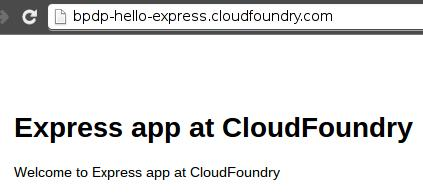
\includegraphics[scale=0.5]{images/bpdp-hello-express.jpg}
    \end{center}
    \caption{Hasil push ke server}
    \label{fig:bab-01-hello}
  \end{figure}

Aplikasi yang sudah dibuat seringkali diubah, oleh karena itu vmc juga menyediakan fasilitas untuk Mengupdate aplikasi. 

\lstset{language=Javascript,caption=Update: menambahkan versi Node.js ke routes/index.js}
\lstinputlisting{src/bab-01/hello/routes/index.js}

\lstset{language=bash,caption=Mengupdate aplikasi di server}
\lstinputlisting{src/non-nodejs/bab-01/update-aplikasi-cf.txt}

Hasilnya bisa dilihat di Gambar~\ref{fig:bab-01-hello-update}

  \begin{figure}
    \begin{center}
      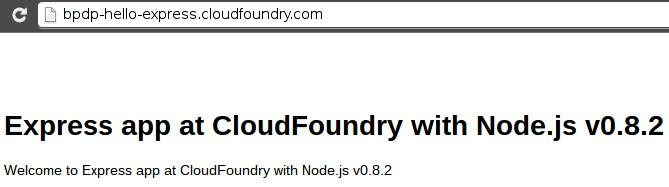
\includegraphics[scale=0.5]{images/bpdp-hello-express-update.jpg}
    \end{center}
    \caption{Hasil update dengan menyertakan versi Node.js}
    \label{fig:bab-01-hello-update}
  \end{figure}

Untuk menghapus aplikasi:

\lstset{language=bash,caption=Menghapus aplikasi yang di-deploy di CF}
\lstinputlisting{src/non-nodejs/bab-01/delete-aplikasi-cf.txt}

Pada saat deployment, kita juga bisa memilih versi Node.js (runtime) sebagai berikut:

\lstset{language=bash,caption=Deployment ke CF dengan memilih runtime Node.js}
\lstinputlisting{src/non-nodejs/bab-01/deploy-pilih-runtime-cf.txt}


Hasilnya bisa dilihat di Gambar~\ref{fig:bab-01-hello-ganti-runtime}

  \begin{figure}
    \begin{center}
      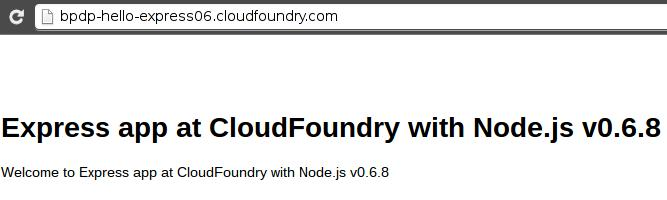
\includegraphics[scale=0.5]{images/bpdp-express-hello-update06.jpg}
    \end{center}
    \caption{Deployement menggunakan versi runtime tertentu}
    \label{fig:bab-01-hello-ganti-runtime}
  \end{figure}

\subsection{Tanpa Framework}

Tanpa \textit{framework}, yang kita perlukan hanyalah langsung mem-\textit{push} file yang kita buat (dalam contoh ini adalah app.js):

\lstset{language=Javascript,caption=app.js tanpa framework}
\lstinputlisting{src/bab-01/hello-no-framework/app.js}

Proses deployement adalah sebagai berikut:

\lstset{language=bash,caption=Deployment app.js tanpa framework}
\lstinputlisting{src/non-nodejs/bab-01/deploy-appjs-no-framework.txt}

Hasilnya bisa dilihat pada Gambar~\ref{fig:bab-01-hello-no-framework}

  \begin{figure}
    \begin{center}
      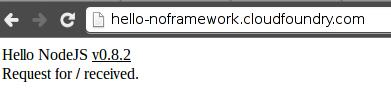
\includegraphics[scale=0.5]{images/hello-noframework.jpg}
    \end{center}
    \caption{Hasil deployement app.js tanpa framework}
    \label{fig:bab-01-hello-no-framework}
  \end{figure}
